\subsubsection{Heavy-flavour correlations}
Although heavy quarks at the LHC energies are mostly produced in primary hard scatterings between the incoming partons in hadronic collisions, a non negligible fraction of c and b quarks are originated in processes of gluon splitting. At the leading order, $\rm c\overline c$ pairs are produced with an azimuthal opening angle of 180$^\circ$. At the next to leading order, gluon splitting and flavour excitation processes can generate $\rm c\overline c$ pairs typically at small opening angles. The role of next-to-leading order production is currently poorly understood even in proton-proton collisions \cite{LHCb-PAPER-2012-003,LorentzpaperHF} and introduces sizeable uncertainties in the models for \PbPb collisions. As a result, heavy-ion calculations which use proton-proton generators as baseline can be biased because of the different energy loss of quarks and gluons. Correlations between D and $\APD$ represent a promising way to study the relevance of these mechanisms in different kinematic ranges of the charm quarks. In \pPb collisions, the study of open heavy-flavour correlations at forward and backward rapidity provides information to test modifications of parton distribution functions in nuclei (see Sect.~\ref{sec:cgctmd}). 

Figure~\ref{fig:DD} shows the LHCb projections for the azimuthal ${\PD \APD}$ correlations at forward rapidity in \pp and \pPb collisions. The figure shows only statistical uncertainties (dominant with respect to the systematic uncertainties) as expected with the Run 3 and 4 integrated luminosity. The measurement of the $\PD \APD$ correlation can be performed in intervals of D meson $\pT$, providing differential information to test theoretical models with precision. The experimental projections are compared with predictions obtained with EPOS3-HQ event generator \textbf{(CURVE MISSING)}. 

In nucleus-nucleus collisions, ${\PD \APD}$ correlations are sensitive observables to discriminate among different mechanisms of in-medium energy loss of heavy-quarks, like radiative and collisional processes. Such measurements, presently challenged by statistical limitations, will greatly benefit from future high-luminosity heavy-ions runs. 

 %These measurements can be complemented with correlation measurements of $\PDz \APDzero$  and $\PDz \PsDm$ as well $\PDz \PGLc^-$, $\PDp \PDm$, $\PDp\PsD-$ and $\PDp \PGLc^-$ as in publication~\cite{LHCb-PAPER-2012-003}.
%The comparison between \pp and \pPb collisions provide information on shadowing and hadronic rescatterings. The knowledge gained from the heavy-flavour correlation studies in small systems is expected to be used to reduce the presently unavoidable uncertainties in the models for \PbPb collisions, providing a more consistent view of the interaction of heavy quarks with the QGP. 
\begin{figure}
\centering
\resizebox{0.5\textwidth}{!}{  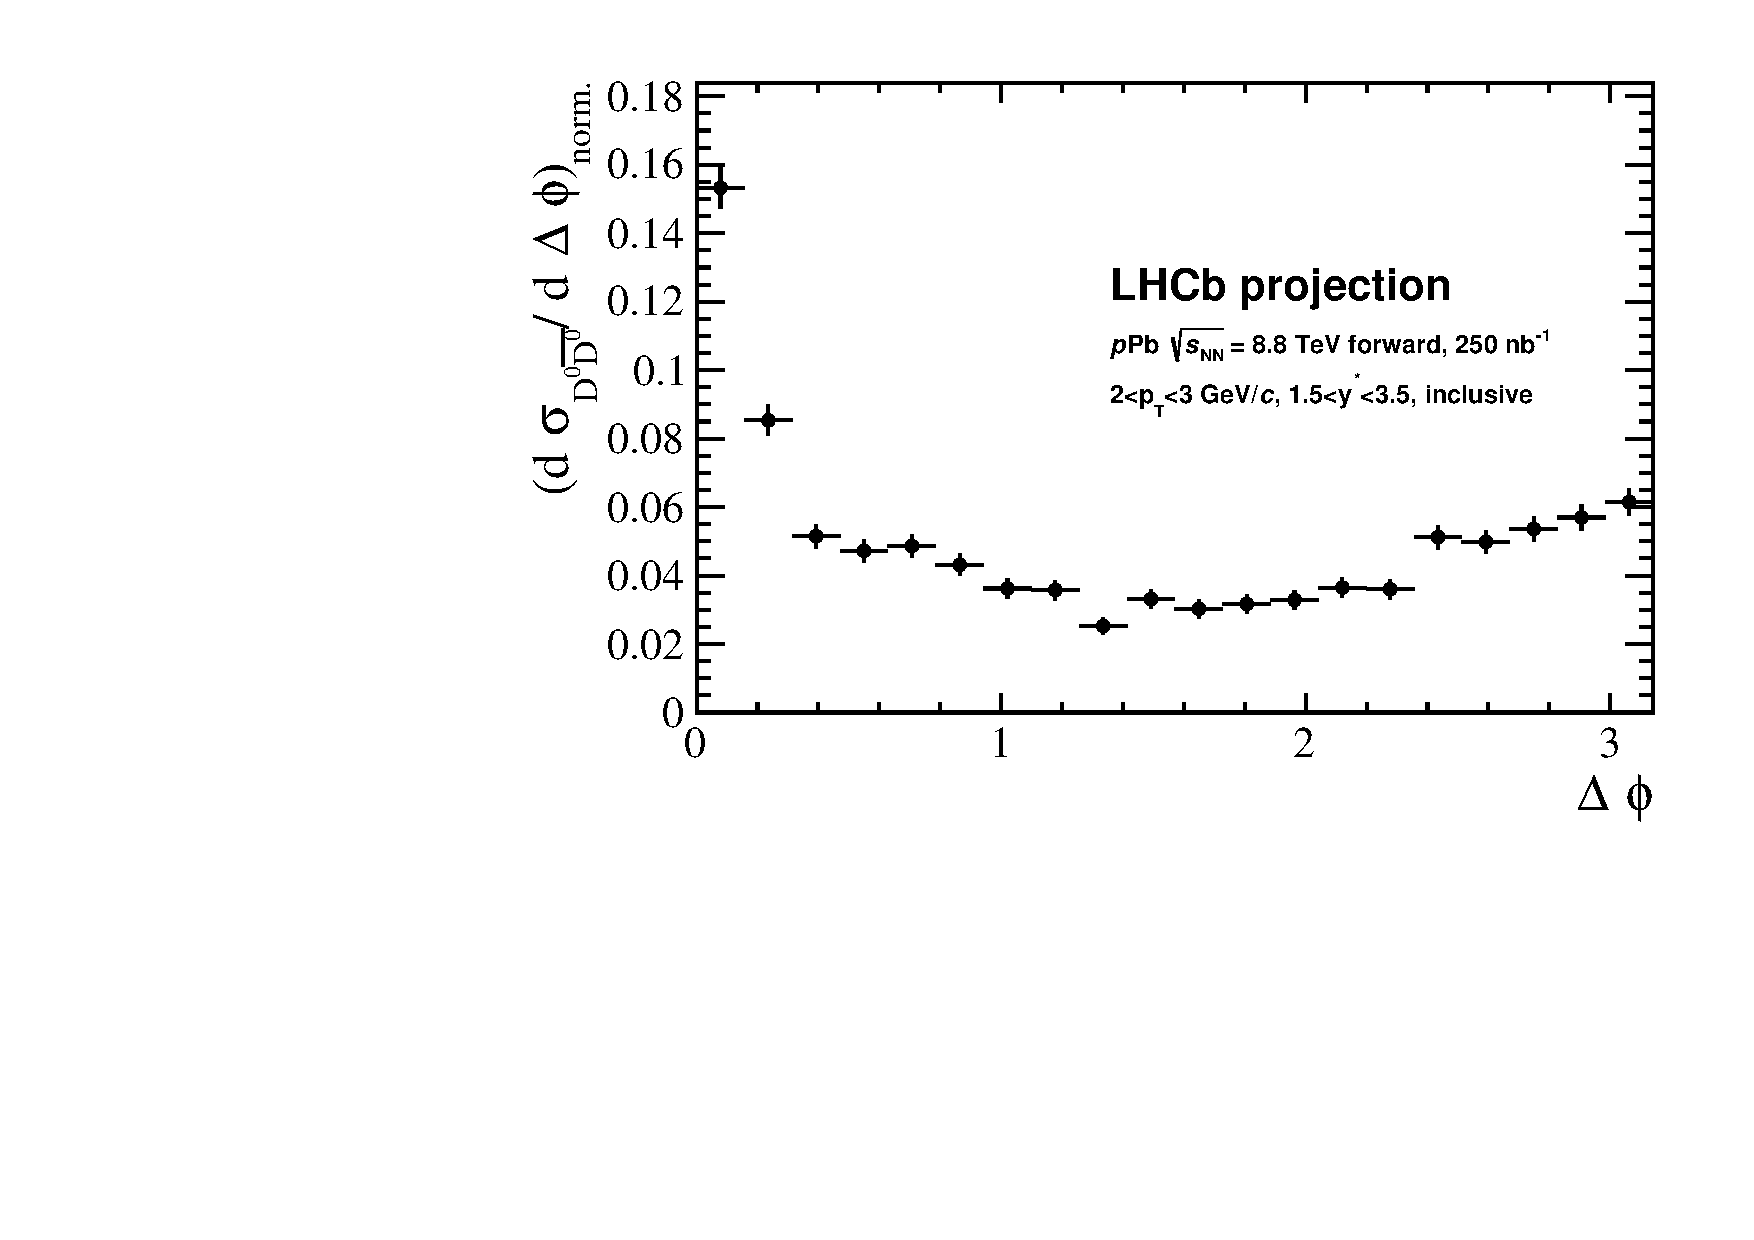
\includegraphics{hf/figures/Deltaphi_pPb_inclusive.pdf}}
\caption{(PLACEHOLDER) LHCb projection of the azimuthal $\PD \APD$ correlations in \pp collisions at $\sqrts=$ 7 $\UTeV$, compared with predictions from the EPOS3-HQ event generator.}
\label{fig:DD}
\end {figure}


\subsubsection{Heavy-flavour jet measurements}
Further insights into the mechanism of parton energy loss in the QGP can be provided by the study of reconstructed heavy-flavour jets. These measurements provide complementary information to the studies of D and B mesons since they allow us to get closer to the energy of the initial heavy quark and give access to the jet energy profile. By comparing the production of heavy-flavour jets with light jets one can test the expected flavour dependence of the in-medium energy loss in a wide transverse momentum range and study the different energy loss mechanism of quarks and gluons. The study of more differential observables related to the production of heavy-flavour particles in jets, like the fragmentation function and the angular correlations, provides additional constraints into the mechanisms of redistribution of the energy lost by the parton inside the medium. %The comparison with the results obtained for the correlations of jets with light hadrons also gives a powerful tool to study the presence of medium-response phenomena caused by the effect of a high $\pT$ jet in the QGP. 


Figure~\ref{fig:DjetCMS} (left) shows the projections for the nuclear modification factor of $\PDzero$-meson tagged jets in \PbPb collisions at $\sqrtsNN=5.02~{\UTeV}$ with ALICE. The measurement will provide a precise estimation of the suppression of $\PDzero$-tagged jets down to low $\pT$, opening the way to study possible modifications of charm fragmentation. Future measurements of the fragmentation functions of charmed hadrons in \pp collisions will also help to reduce the uncertainties on the charm fragmentation mechanisms, which are currently among the main sources of uncertainties for theoretical calculations that describe heavy-quark observables at the LHC. 

Figure~\ref{fig:DjetCMS} (right) shows the projections for the distributions of $\PD$ mesons as a function of the distance from the jet axis for jets of $\pT>$~60~$\UGeV$ in \pp and \PbPb collisions at $\sqrtsNN=5.02~{\UTeV}$. In the same figure, the ratio of the $\PDzero$ radial distribution of \PbPb to \pp are also presented in the bottom panel of the figure. With the precision achievable with the high-luminosity data, one would be able to measure precisely the effect of heavy-quark in-medium energy loss and the redistribution of the energy at large angle with respect to the jet axis. This is expected to provide new constraints on in-medium energy loss calculations. By comparing the ratio measured for D mesons with the one obtained for charged particles, it will be possible to assess the relevance of medium response phenomena, which can induce modification of the jet shape at large angles and are expected to be less relevant for heavy quarks due to their large masses \textbf{(CITE JET CHAPTER)}.

\begin{figure}
\centering
\resizebox{0.45\textwidth}{!}{  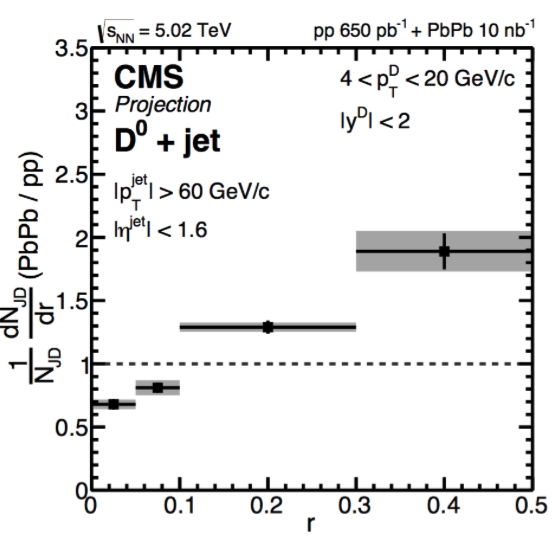
\includegraphics{hf/figures/DjetCMS}}
\resizebox{0.45\textwidth}{!}{  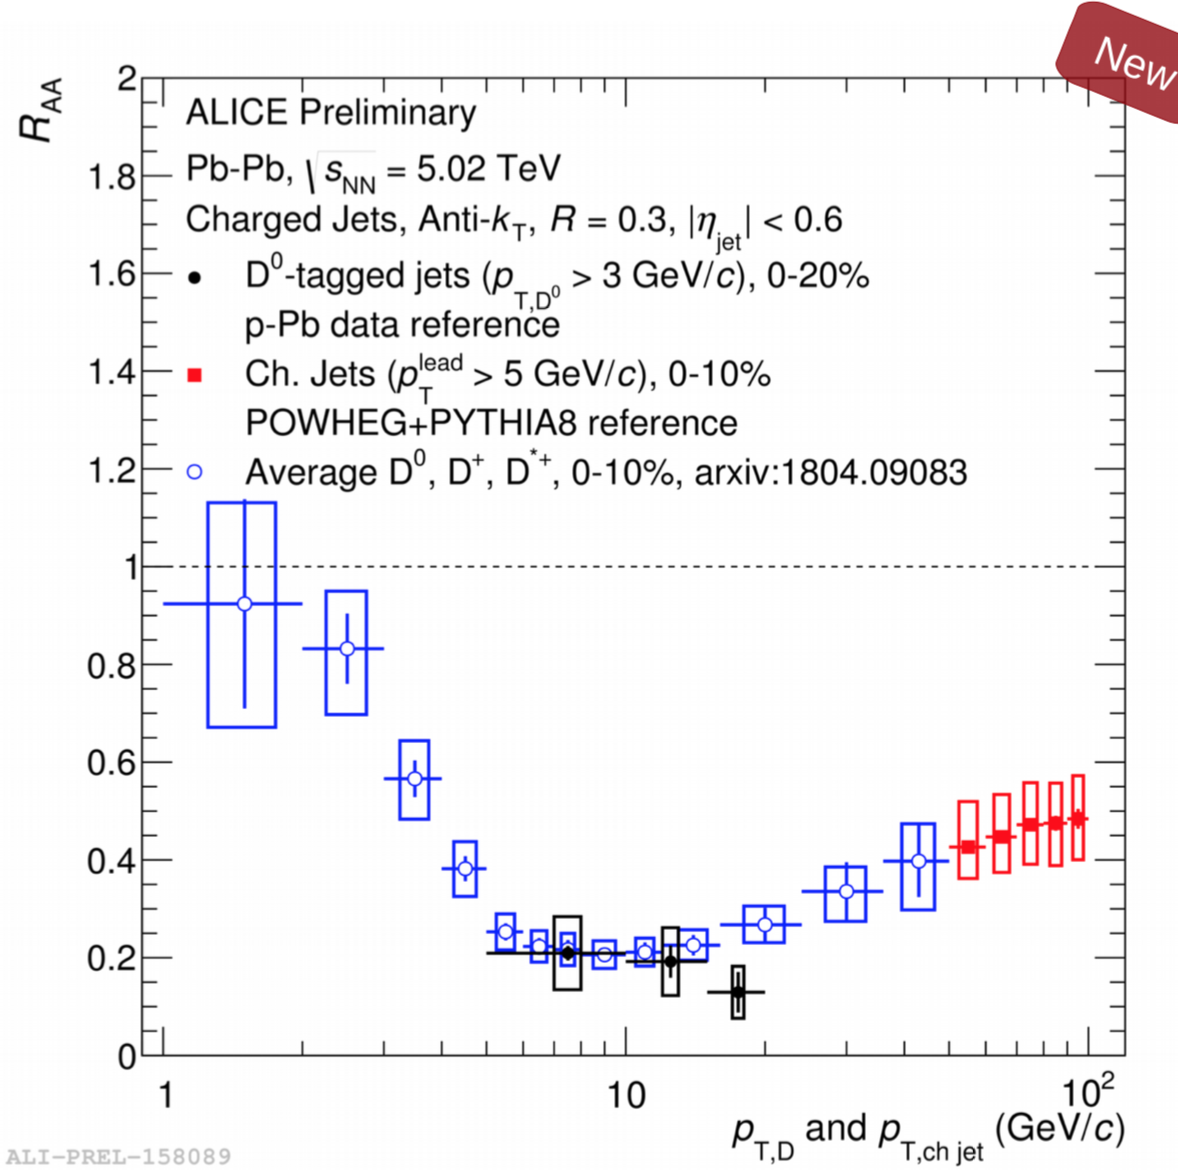
\includegraphics{hf/figures/DTaggedJetALICE}}
\caption{(Left) Distributions of $\PD$ mesons in jets as a function of the distance from the jet axis for jets of $\pT>$60 GeV in \pp and \PbPb collisions at $\sqrtsNN=5.02~{\UTeV}$. The ratio of the $\PDzero$ radial distribution of \PbPb to \pp is also presented in the bottom panel of the figure. (Right) Nuclear modification factor of $\PDzero$-meson tagged jets in 0--20$\%$ \PbPb collisions compared to the average prompt D-meson $\RAA$.}
\label{fig:DjetCMS}
\end {figure}

\subsubsection{Heavy-flavour jet substructure}

Another area of research where the LHC experiments can make key contributions is the study of heavy-flavour jet substructure. New experimental observables related to the inner structure of heavy-flavour jets, like the splitting functions\textbf{(CITE JET CHAPTER)}, can provide insights into the mass dependence of the parton shower in new kinematic regimes. A precise measurement of these observables at the LHC down to low $\pT$ would also provide a unique opportunity to further investigate the dead cone effect~\cite{DOKSHITZER2001199}, currently not well understood and constrained.

